\chapter{感情プロトタイプを超えた共有情動変調軸}
\label{chap:development2_preverbal_vectors}

前章では、特定の目標感情 $e$ に対して、感情固有の残差ベクトル $\hat{\mathbf{r}}_e$ が十分かつ信頼性の高いステアリング信号であることを示した。パラメータスイープにより、共有された感情化成分 $\mathbf{g}$ はテストしたすべてのスケールで逆効果であることが実証された。すなわち、$\mathbf{g}$ を加えると目標感情マッチ度、意味保存性、および出力の感情性がいずれも低下する。したがって、有効な情動ステアリングは次のように集約される。
\[
\Delta_e = \alpha_R\,\hat{\mathbf{r}}_e,
\]
ここで $\alpha_G$ 係数は破棄される。しかし、$\hat{\mathbf{r}}_e$ は目標とする感情を制御するに過ぎず、その感情がどのように表現されるかには関与しない。本章では、残差ストリームが感情ラベルとは独立して表現のテクスチャを調整する別の情動変調レイヤーをエンコードしているかどうか、そしてもしそうであれば、それを因果的にステアリングできるかどうかを問う。\par

そのフレームワークにおいて、\textit{joy}、\textit{sadness}、\textit{anger}、その他のプルチック分類は原始的な単位として扱われてきた。各 $\hat{\mathbf{r}}_e$ はそれ以上の分解を行わない、原子的な感情固有ベクトルとみなされていた。\par

本章ではその仮定を再検討する。中心的な問いは、命名された感情カテゴリがモデルの残差ストリームにおける情動表現の最小単位であるか、あるいは各 $\hat{\mathbf{r}}_e$ の周辺のコーンが、より基本的な前カテゴリ的な情動次元の小さな集合を含んでいるかどうかである。ここで報告する実験は後者の証拠を提供する。すなわち、単一の命名された感情内で変化する部分軸が感情カテゴリ間で系統的に再現されており、それらが命名された感情ラベルよりも原始的であることを示唆する。\par

感情内残差部分空間、すなわち $\hat{\mathbf{r}}_e$ を射影除去した後に残る活性化空間の部分が、共有された情動軸 $\mathbf{m}_k$ の小さな集合によって組織されていることを見出した。$\mathbf{m}_k$ は $\hat{\mathbf{r}}_e$ を既に射影除去した部分空間から抽出されているため（Section~\ref{sec:ch2-meta-axes}）、構成上感情プロトタイプと直交している。それら自体は $\hat{\mathbf{r}}_e$ を分解するのではなく、コーン領域内で情動表現を調整する\textbf{補助変調軸}として機能する。完全なステアリング信号は次のようになる。
\[
\Delta_e \;=\; \alpha_R\,\hat{\mathbf{r}}_e \;+\; \sum_{k}\gamma_k\,\mathbf{m}_k,
\]
ここで $\alpha_R$ は目標感情を選択し、$\gamma_k$ は各前言語的軸に沿って情動テクスチャを独立に変調する。$\mathbf{m}_k$ が因果的に活性であるか（$\gamma_k \neq 0$ を設定することで感情ラベルを変えずに表現テクスチャをシフトするか）は Section~\ref{sec:ch2-causal-validation} で検証する。\par


\section*{実験ロードマップ}

本章は以下のように構成されている。
\begin{enumerate}
  \item \textbf{内部分散構造}：各命名感情の内部次元性を、各感情カテゴリ内のソースごとの残差ベクトルの分布に主成分分析（PCA）を適用することで特徴付ける。
  \item \textbf{プールドPCAによる共有メタ軸}：感情ごとのプールドPCAが、感情ごとの別々のPCAや符号整合を必要とせず、共有メタ軸 $\mathbf{m}_k$ の集合を直接回復することを示す。
  \item \textbf{前言語的解釈}：すべての感情から同時に極端な例を大規模言語モデル（LLM）に提示することで各 $\mathbf{m}_k$ を解釈し、各メタ軸に対して感情に依存しない意味ラベルを取得する。
  \item \textbf{活性化ステアリングによる因果的検証}：$\gamma\,\mathbf{m}_k$ を様々なスケールで残差ストリームに直接注入し、情動テクスチャの結果的なシフトを測定することで $\mathbf{m}_k$ が因果的に活性であることを検証し、そのシフトが感情カテゴリの置換ではなくテクスチャレベルに留まるかどうかをテストする。
\end{enumerate}

\section{命名感情の内部分散構造}
\label{sec:ch2-variance-structure}

Chapter~\ref{chap:development1_emo_steering} では、$\hat{\mathbf{r}}_e$ が有効な感情固有信号であることが確立された。共有された感情化成分 $\mathbf{g}$ を残差化した後、8つの残差方向はプルチック様の幾何学を回復し（隣接--対立コサインギャップが $0.010$ から $0.041$ へと拡大）、線形プローブは $93.8\%$ の8クラス精度を達成する（Section~\ref{sec:decomposition_validity}）。\par

しかし、$\hat{\mathbf{r}}_e$ は同じ感情に対する多くの個別ソース残差シフト $\boldsymbol{\delta}^{g\perp}_{n,e,i}$ の平均である。これらのシフトは平均方向の周辺に密集するかもしれないし、いくつかの異なる方向に広がるかもしれない。本セクションでは、その感情内分布の形状を調べ、各命名感情が単一ベクトルで十分に記述されるか、あるいは残差空間においてより広い多次元領域を占めるかを問う。\par

\subsection*{プロトコル}

各感情 $e$ について、層~13におけるソースごと・強度ごとの残差 $\boldsymbol{\delta}^{g\perp}_{n,e,i}$ を収集し、主成分分析（PCA）~\cite{pearson1901pca}を適用して参加比率を計算する。
\[
\mathrm{PR}_e
=\frac{\left(\sum_k \lambda_k\right)^2}{\sum_k \lambda_k^2},
\]
ここで $\lambda_k$ は経験的共分散の固有値である。
ベースラインを確立するため、感情固有の構造を破壊するように感情ラベルをシャッフルし、$\mathrm{PR}_{\mathrm{shuffle}}$ を報告する。$\mathrm{PR}_e < \mathrm{PR}_{\mathrm{shuffle}}$ の値は感情の内部分布がランダムよりも集中していることを示し、$\mathrm{PR}_e > \mathrm{PR}_{\mathrm{shuffle}}$ はより拡散した多軸構造を示す。\par

\subsection*{結果}

% Table: participation ratio (from exp2)
\begin{table}[H]
\centering
\small
\begin{tabular}{lccc}
\toprule
\textbf{感情} & \textbf{PR} & \textbf{PR（シャッフル）} & \textbf{PR超過量} \\
\midrule
joy        &  6.72 & 13.62 & $-6.90$ \\
trust      & 10.54 & 13.65 & $-3.11$ \\
sadness    & 12.11 & 13.59 & $-1.48$ \\
disgust    & 12.74 & 13.61 & $-0.87$ \\
anticipation & 15.30 & 13.65 & $+1.65$ \\
anger      & 15.56 & 13.63 & $+1.93$ \\
fear       & 18.16 & 13.60 & $+4.57$ \\
surprise   & 18.94 & 13.63 & $+5.31$ \\
\bottomrule
\end{tabular}
\caption{層~13におけるソースごとの情動シフト分布の参加比率。負の超過量は一軸近似構造を示し、正の超過量は多軸構造を示す。}
\label{tab:exp2_participation_ratio}
\end{table}

結果は感情カテゴリ間に明確な勾配を示す。\textit{joy}と\textit{trust}は最も集中している。それらのPR値（$6.72$ と $10.54$）はシャッフルベースライン（$\approx 13.6$）を大幅に下回り、感情内の一軸近似構造を示す。対照的に、\textit{fear}と\textit{surprise}は著しく拡散している。それらのPR値（$18.16$ と $18.94$）はシャッフルベースラインを $+4.57$ と $+5.31$ 上回り、それらの残差が複数の軸にわたることを示す。\par

\begin{figure}[H]
  \centering
  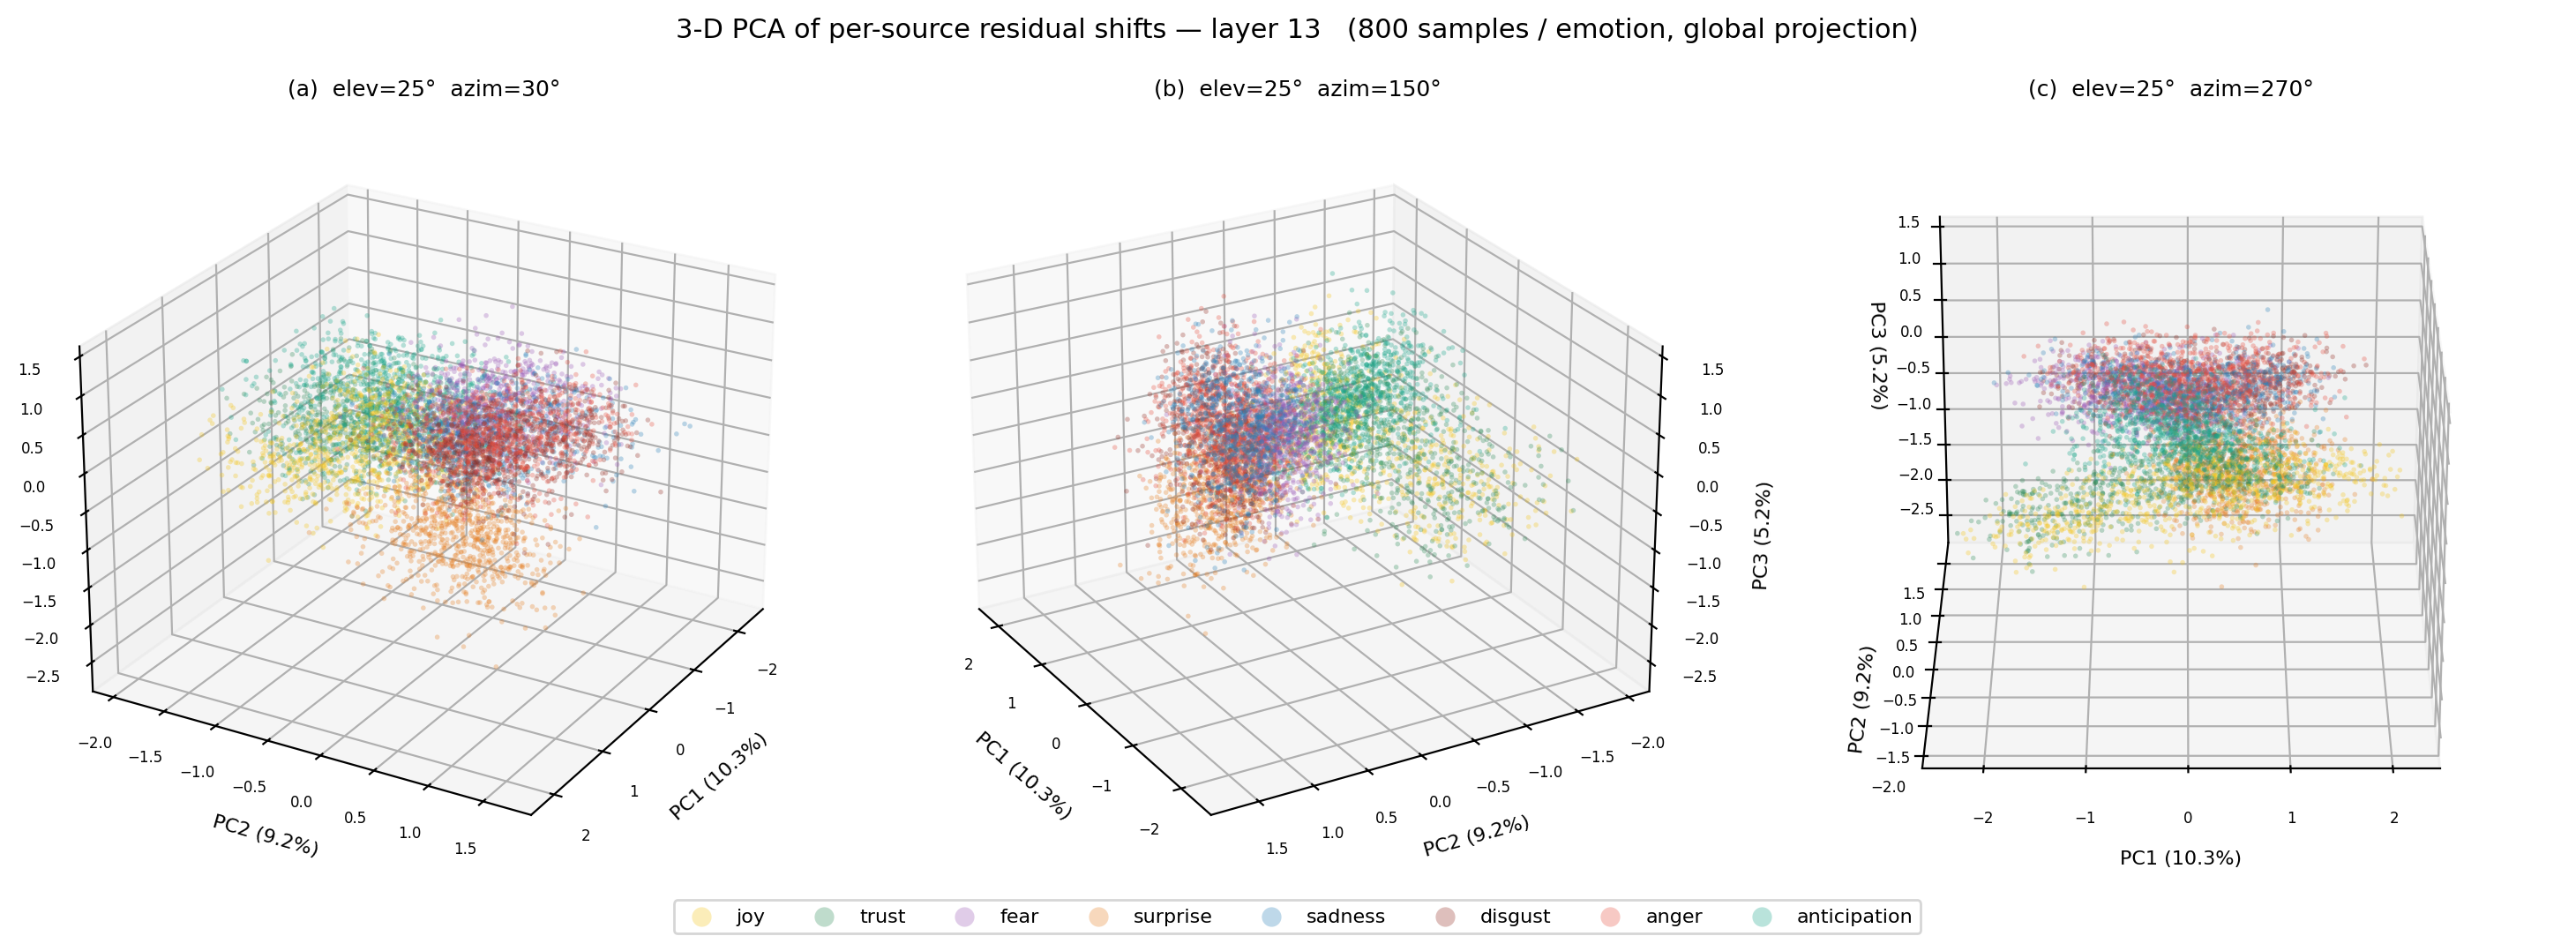
\includegraphics[width=0.8\linewidth]{figures/pca3d_residuals.png}
  \caption{層13におけるソースごとの情動残差シフトの3D主成分分析（PCA）射影。このプロットは感情カテゴリ間の集中--拡散の違いを可視化している。}
  \label{fig:exp2_pca3d_residuals}
\end{figure}

この集中--拡散の違いは、ソースごとの残差シフトの3D PCA射影に直接見て取れる（Figure~\ref{fig:exp2_pca3d_residuals}）。\textit{joy}と\textit{trust}がコンパクトな雲のような分布を形成するのに対し、\textit{fear}と\textit{surprise}は共有座標系のより広い領域に広がっている。\par

\begin{figure}[H]
  \centering
  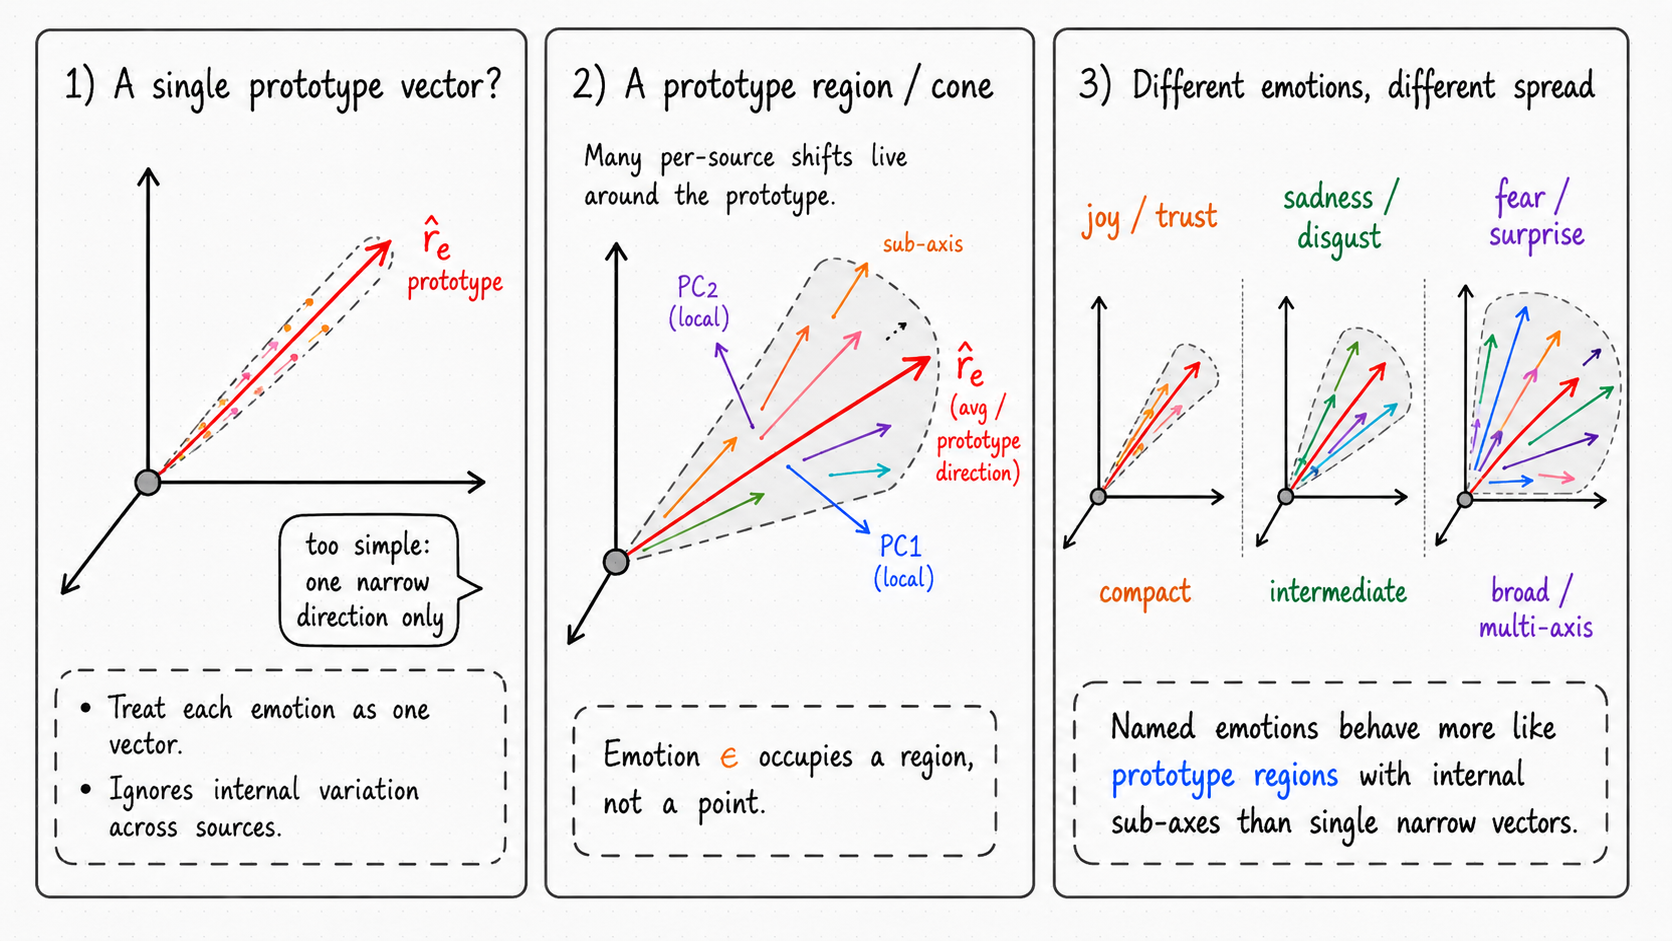
\includegraphics[width=0.75\linewidth]{figures/prototype_region.png}
  \caption{命名感情のプロトタイプ領域の解釈。命名感情は単一の平均方向 $\hat{\mathbf{r}}_e$ だけでなく、そのプロトタイプ周辺のソースごとの残差シフトの分布によって表現される。この領域の幅は感情間で異なり、コンパクトな感情もあれば、より豊かな内部部分軸を含む感情もあることを示唆する。}
  \label{fig:exp2_prototype_region}
\end{figure}

これらの結果を総合すると、命名感情は内部次元性において異なることが分かる。一部（\textit{joy}、\textit{trust}）は単一ベクトルで十分に捉えられるが、他（\textit{fear}、\textit{surprise}）はより広い多軸領域を占める。したがって、$\hat{\mathbf{r}}_e$ は感情 $e$ の有用な重心を提供するが、各命名感情は単一の狭いベクトルよりも内部部分軸を持つコーンとして特徴付けられる。\par

% ─────────────────────────────────────────────────────────────
\section{プールドPCAによる共有メタ軸}
\label{sec:ch2-meta-axes}

Section~\ref{sec:ch2-variance-structure} の参加比率分析により、各感情の残差は単一ベクトル方向ではなく多次元領域を占めることが確立された。次に、それらの次元が感情固有のものか、それともすべての感情カテゴリにわたって再現されるかを調べる。これにより、$\hat{\mathbf{r}}_e$ が真の原子的ベクトルであるか、それとも共有情動部分空間への射影であるかが決まる。\par

$\mathbf{u}_{e,k}$ を感情 $e$ だけの残差の第 $k$ 主成分とし、$\mathbf{u}_{e,1}$ を先頭の感情内分散方向、$\mathbf{u}_{e,2}$ を2番目とする。対応する固有値 $\lambda_{e,k}$ は $\mathbf{u}_{e,k}$ に沿った感情 $e$ の残差分散を測定する。\par

感情ごとに別々にPCAを実行すると、各感情の内部分散構造を捉えるローカル固有ベクトル $\{\mathbf{u}_{e,k}\}_{k}$ が得られる。しかし、これらの感情ごとの分解は直接比較できない。\textit{joy}の第 $k$ 固有ベクトルが\textit{sadness}の第 $k$ 固有ベクトルに対応する必要はなく、それらの順序は各感情ブロック内で独立して決定されるからである。\par

本セクションを通じて、$\mathbf{u}_{e,k}$ は単一感情ブロック内でフィットされたPCAからのローカルPCを示し、$\lambda_{e,k}$ はその関連固有値を示し、$\tilde{\mathbf{m}}_k$ はスタックされた残差行列にフィットされた単一のPCAから得られるプールドPCを示す。\par

\subsection{プールドPCAの直感}

ベクトル $\mathbf{v}$ が8つすべての感情にわたって共有されており、各 $e$ に対して固有値 $\lambda_{e,1}$ で各感情の共分散の先頭固有ベクトルとして現れると仮定する。$\Sigma_{\mathrm{pool}}$ への寄与は次のようになる。
\[
\sum_{e} \lambda_{e,1}\,\mathbf{v}\mathbf{v}^\top
= \Bigl(\lambda_{\mathrm{joy},1} + \lambda_{\mathrm{sadness},1} + \lambda_{\mathrm{anger},1} + \cdots\Bigr)\mathbf{v}\mathbf{v}^\top.
\]
スカラープレファクタはすべての感情からの固有値を蓄積する。具体的に、各 $\lambda_{e,1} = 10$ とすると、共有方向 $\mathbf{v}$ はプールドスペクトルに $10 \times 8 = 80$ を寄与する。\par

対照的に、ベクトル $\mathbf{w}$ が1つの感情（例：\textit{anger}）に固有である場合、$\mathbf{u}_{\mathrm{anger},2} \approx \mathbf{w}$ で、他の感情は $\mathbf{w}$ に沿って無視できる分散を持つとする。そのプールドへの寄与は次のようになる。
\[
\lambda_{\mathrm{anger},2}\,\mathbf{w}\mathbf{w}^\top,
\]
単一の項である。$\lambda_{\mathrm{anger},2} = 10$ であっても、感情固有方向は $10 \times 1 = 10$ しか寄与せず、共有方向の重みの8分の1である。$\mathbf{w}$ のプールド固有値は感情横断的なサポートの欠如によって抑制される。\par

この非対称性により、単一のプールドPCAは共通性の検出器となる。共有軸は線形蓄積によってスペクトルの上位に昇格し、感情固有軸は低次成分に希釈される。プールドされた残差に適用された単一のPCAは、感情ごとの別々のPCAや符号整合を必要とせず、すべての感情にわたって一貫してサポートされる分散方向を優先的に回復する。\par

\subsection{プロトコル}

各感情 $e$ について、4ステップパイプラインによって得られた前処理済み残差 $\{\boldsymbol{\delta}^{(3)}_{n,e,i}\}_{n,i}$ を収集する。
\begin{enumerate}
  \item 活性化シフト $\boldsymbol{\delta}_{n,e,i} = \mathbf{h}^{\mathrm{emo}}_{n,e,i} - \mathbf{h}^{\mathrm{neu}}_{n}$ を計算する
  \item 共有された感情化方向 $\mathbf{g}$ を射影除去する
  \item 感情ごとのプロトタイプ $\hat{\mathbf{r}}_e$ を射影除去する
  \item トピックとスタイルの交絡因子を除去するためにソースごとの感情全体の平均を減算する
\end{enumerate}

次に各感情ブロックを中心化し、すべてのブロックを単一の $(N \cdot E,\, D)$ 行列にスタックして主成分分析（PCA）を適用する。得られた成分 $\{\tilde{\mathbf{m}}_k\}$ が候補メタ軸である。\par

\subsection{結果}

\subsubsection*{説明分散}
上位3つのプールド成分は、総プールド分散の $11.4\%$、$4.5\%$、$3.1\%$ を占める（累積 $\approx 19.0\%$）。第1成分が著しく優勢で、第2成分の2倍以上の分散を説明しており、単一の主要な共有次元が存在することを示す。\par

\subsubsection*{メタ軸との整合性}
プールド成分が真の感情横断的構造を捉えていることを検証するために、それらを符号整合平均メタ軸 $\mathbf{m}_k$ と比較する。これは符号補正後に感情にわたって正規化平均された感情ごとの第 $k$ 固有ベクトルとして定義される。具体的には、$\sigma_{e,k}\in\{+1,-1\}$ が感情にわたって平均化する前に各固有ベクトルの任意の符号を補正する。
\[
\mathbf{m}_k
=\frac{\sum_{e\in E}\sigma_{e,k}\,\mathbf{u}_{e,k}}
      {\left\lVert\sum_{e\in E}\sigma_{e,k}\,\mathbf{u}_{e,k}\right\rVert_2}.
\]
プールド成分 $\tilde{\mathbf{m}}_k$ は先頭3成分について個別軸レベルで $\mathbf{m}_k$ とほぼ完全に一致する（Table~\ref{tab:pooled_vs_meta}、Figure~\ref{fig:pooled_robustness}）。\par

\begin{table}[H]
\centering
\small
\begin{tabular}{lc}
\toprule
\textbf{比較} & $|\cos(\tilde{\mathbf{m}}_k,\,\mathbf{m}_k)|$ \\
\midrule
$\tilde{\mathbf{m}}_1$ vs.\ $\mathbf{m}_1$ & 0.988 \\
$\tilde{\mathbf{m}}_2$ vs.\ $\mathbf{m}_2$ & 0.980 \\
$\tilde{\mathbf{m}}_3$ vs.\ $\mathbf{m}_3$ & 0.931 \\
\bottomrule
\end{tabular}
\caption{層~13におけるプールドPCA成分 $\tilde{\mathbf{m}}_k$ と符号整合平均メタ軸 $\mathbf{m}_k$ の間の絶対コサイン類似度。上位3つのスパンにわたる部分空間相互捕捉率は $96.6\%$ である。}
\label{tab:pooled_vs_meta}
\end{table}

\begin{figure}[H]
  \centering
  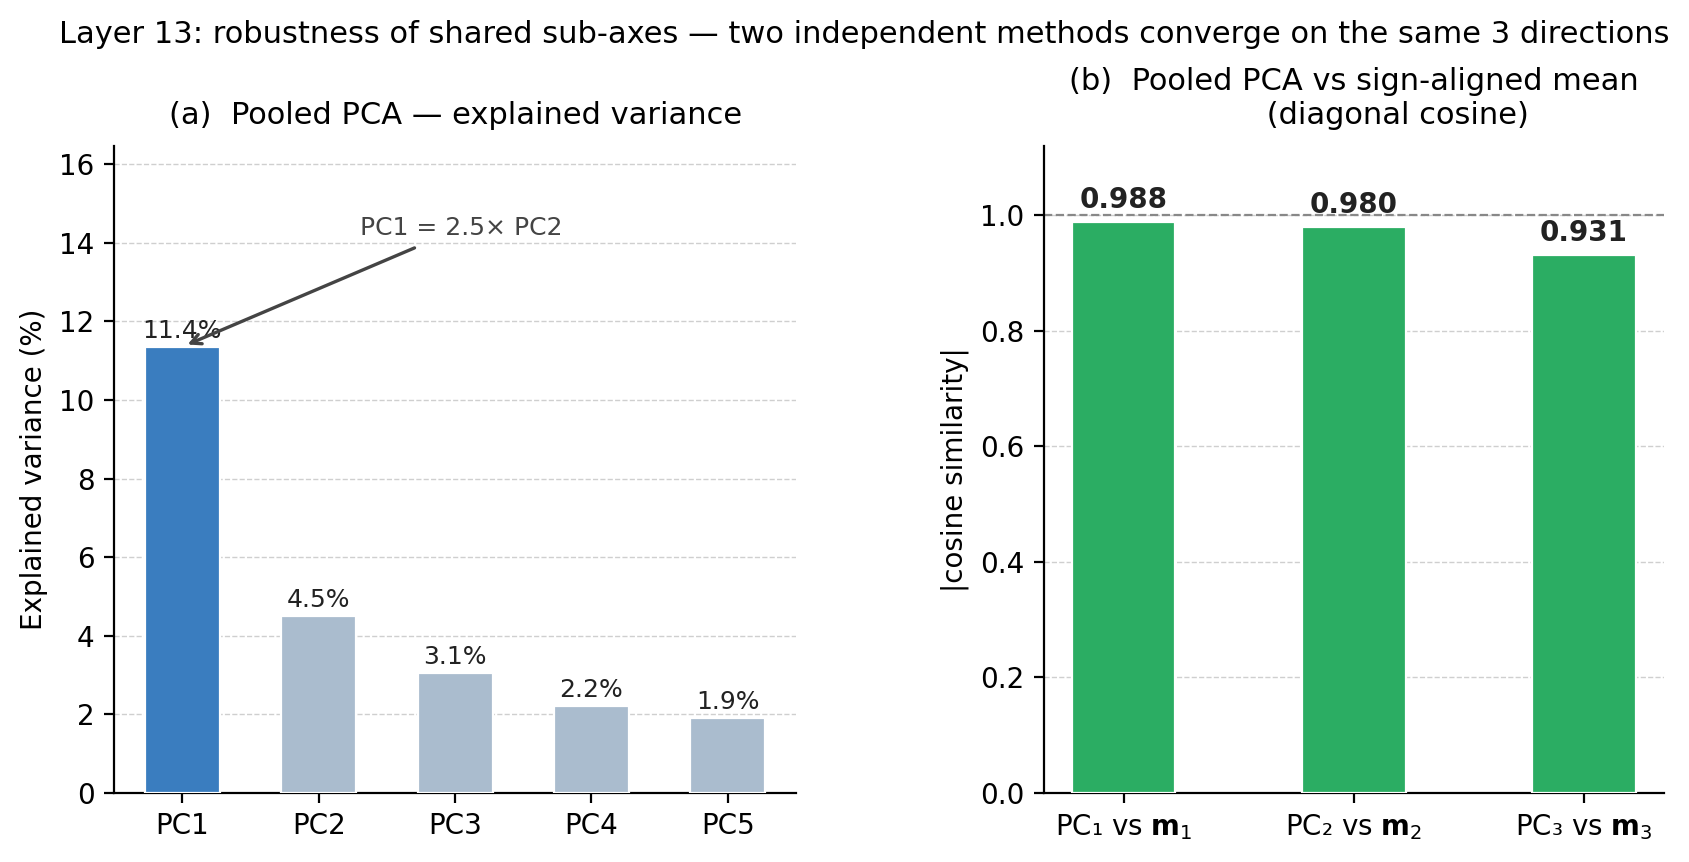
\includegraphics[width=0.7\linewidth]{figures/pooled_robustness.png}
  \caption{層~13におけるプールドPCAと符号整合平均メタ軸の収束。\textbf{(a)} スクリープロット：PC$_1$ は総分散の $11.4\%$ を占め、第2成分の $2.5\times$ 以上であり、1つの強く支配的な共有方向が存在することを示す。\textbf{(b)} 各プールド成分 $\tilde{\mathbf{m}}_k$ と対応するメタ軸 $\mathbf{m}_k$ の対角コサイン類似度。3つすべての値が $0.93$ を超えている。}
  \label{fig:pooled_robustness}
\end{figure}

\begin{figure}[H]
  \centering
  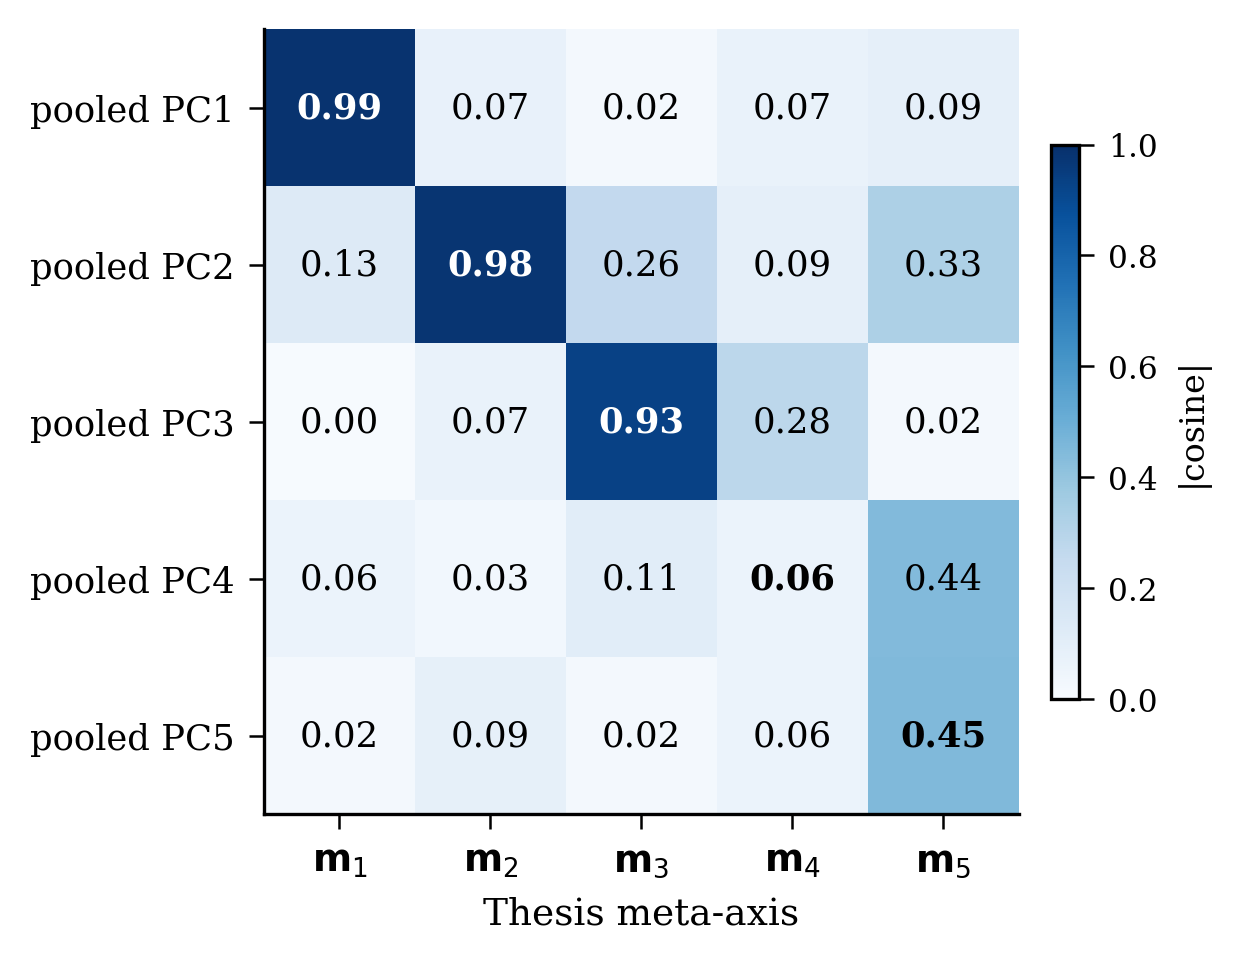
\includegraphics[width=0.55\linewidth]{figures/pooled_mk_heatmap.png}
  \caption{層~13におけるプールドPCA成分と符号整合平均メタ軸 $\mathbf{m}_k$ の間の完全な $5\times 5$ 絶対コサイン行列。左上の $3\times 3$ ブロックは強く対角的であり（対角 $\geq 0.93$）、対応関係が単なる部分空間レベルではなく軸レベルであることを確認している。PC$_4$--PC$_5$ の行はいずれの $\mathbf{m}_k$ に対しても $0.50$ を超える実質的な整合性を示さない。}
  \label{fig:pooled_mk_heatmap}
\end{figure}

完全な $3\times 3$ コサイン行列の非対角エントリはほとんど小さく、プールドPCAが共有部分空間だけでなく各個別軸を再現していることを確認している。上位3スパンにわたる部分空間相互捕捉率は $96.6\%$ である。\par

\subsubsection*{$\mathbf{m}_k$ の幾何学的性質}
3つのメタ軸はさらに2つの幾何学的性質を満たす。第一に、すべての $\mathbf{m}_k$ は共有された感情化方向 $\mathbf{g}$ とほぼ直交している（すべての $k$ について $|\cos(\mathbf{m}_k,\mathbf{g})| < 0.02$）。第二に、すべての感情ごとのプロトタイプ $\hat{\mathbf{r}}_e$ とほぼ直交している（すべての $k,e$ について $|\cos(\mathbf{m}_k,\hat{\mathbf{r}}_e)| < 0.09$）。第二の性質は偶然ではない。これはPCAを適用する前にステップ~3で $\hat{\mathbf{r}}_e$ を射影除去し、構成上プロトタイプと直交する部分空間に $\mathbf{m}_k$ を閉じ込める抽出手順から直接導かれる。Appendix~\ref{app:ablation}（A1）はこのステップが本質的であることを支持する証拠を提供している。プロトタイプ除去なしでは先頭のプールド成分が大域的感情化方向に崩落する。したがって各メタ軸は感情のアイデンティティではなく情動テクスチャを捉えている。すなわち、どの感情がアクティブであるかとは独立に、離散感情がどのように表現されるかの連続的変化である。これらの性質を総合すると、$\mathbf{m}_k$ 基底が大域的感情化軸と感情ラベル方向の両方から幾何学的に独立しており、プロトタイプ平均化が捨てる感情内分散を回復していることが確認される。\par

成分 $\tilde{\mathbf{m}}_4$ と $\tilde{\mathbf{m}}_5$ は低い手法間安定性を示す。各々は $2.2\%$ 未満の分散を説明し、対応する符号整合平均軸との相互捕捉率は $0.50$ を下回り、PC$_4$--PC$_5$ はすべての $\mathbf{m}_k$ に対して $\leq 0.45$ のコサイン類似度を示す（Figure~\ref{fig:pooled_mk_heatmap}）。したがって、3つの安定した軸（$\mathbf{m}_1$、$\mathbf{m}_2$、$\mathbf{m}_3$）と2つの低安定性軸（$\mathbf{m}_4$、$\mathbf{m}_5$）を区別する。$\mathbf{m}_4$ と $\mathbf{m}_5$ は幾何学的に低安定性だが、5つすべての軸が Section~\ref{sec:ch2-preverbal-interp}--\ref{sec:ch2-causal-validation} の解釈と因果テストに持ち越される。各軸が因果的に機能するかどうかは幾何学的安定性だけでなくステアリング実験によって解決される経験的問題である。\par

\subsection{ロバスト性：2つの独立した手法の収束}
\label{sec:ch2-pooled-robustness}

Table~\ref{tab:pooled_vs_meta} と Figure~\ref{fig:pooled_robustness} で報告された収束は、意図的なロバスト性テストの結果である。このサブセクションではそのテストの設計を明示し、収束が何を意味するかを述べる。\par

符号整合平均とプールドPCAは根本的に異なる抽出戦略を表している。符号整合平均は最初にデータを感情ラベルで分割する。8つの感情カテゴリそれぞれの中で別々のPCAを実行し、次に結果を順位ごとに符号整合して平均し、すべての段階で感情分割に依存する。プールドPCAは対照的に、各感情ブロックを中心化してその平均を除去してから、スタックされた残差に単一の分解を適用する。中心化ステップは感情ラベルを使用するが、PCA自体はラベルなし行列で動作し、どの観測がどの感情に属するかを参照しない。したがって2つの手法は共有方向をどのように発見すべきかについて独立した構造的仮定をエンコードしている。\par

自然な懸念の1つは、メタ軸が符号整合平均手順のアーティファクトである可能性である。例えば、符号整合ステップや感情ごとの分割が、そうでなければ存在しない構造を押し付けているかもしれない。プールドPCAは符号整合の選択と順位ごとの再結合の両方に対して免疫を持っている。ブロック中心化後、固有値分解中に感情のアイデンティティを参照することなく、スタックされた行列に単一の分解を適用する。それにもかかわらず、同じ3つの方向を回復し、各 $\mathbf{m}_k$ を個別に軸レベルで、また集合的に部分空間レベルで一致させている（Table~\ref{tab:pooled_vs_meta}、Figures~\ref{fig:pooled_robustness}--\ref{fig:pooled_mk_heatmap}）。これにより、$\mathbf{m}_1$、$\mathbf{m}_2$、$\mathbf{m}_3$ のソースとしてそれらの方法論的選択が除外される。\par

内部ステップを共有しない2つの手法が同じ3つの情動軸に収束している。この収束は、$\mathbf{m}_1$、$\mathbf{m}_2$、$\mathbf{m}_3$ が特定の抽出手順のアーティファクトではなく、モデルの残差活性化における真の共有構造を反映しているという最も強力な証拠を構成する。\par

% ─────────────────────────────────────────────────────────────

\section{メタ軸の前言語的解釈}
\label{sec:ch2-preverbal-interp}

次に、共有メタ軸 $\mathbf{m}_k$ がどのような情動情報をエンコードしているかという問いに向かう。命名された感情カテゴリによってインデックス付けられた残差ベクトル $\hat{\mathbf{r}}_e$ とは異なり、$\mathbf{m}_k$ は感情にわたって共有された分散構造から抽出されている。各 $\mathbf{m}_k$ は\textit{joy}、\textit{sadness}、\textit{anger}などの単一の感情ラベルにインデックス付けられておらず、代わりに候補となる\textbf{前言語的情動次元}として扱われる。すなわち、離散カテゴリ割り当ての前に情動体験や表現を変調する方向である。低安定性軸 $\mathbf{m}_4$ と $\mathbf{m}_5$ を含む5つすべての軸を解釈する。これら2つの軸のラベルは暫定的であり、因果的活性は Section~\ref{sec:ch2-causal-validation} で各軸について独立して評価される。\par

これらの方向を解釈するために、対比的な大規模言語モデル（LLM）評価器（\texttt{GPT-4o}）手順を適用する。各メタ軸について、8つすべての感情にわたってプールされた極端な正および負の射影を持つ例を収集し、次に5つすべての軸を同時に審判に提示し、各軸の高極と低極に異なるラベルを割り当てるよう指示する。同時提示は重要である。軸を個別に解釈する場合、支配的な信号は一般的な「関与対回避」や覚醒度様の区別に崩落する傾向があるからである。評価器に軸を互いに比較させることで、すべての情動変化に共有されているものではなく、各軸に固有のものを捉えるラベルを引き出す手順になる。結果を Table~\ref{tab:meta_axis_interpretations} に示す。\par

予備版では各軸を審判に独立して提示した。これにより、すべての軸でほぼ同一のラベル（\textit{関与対回避}または\textit{覚醒対静穏}）に崩落し、独立提示では軸固有のラベルを引き出すには不十分であることが確認された。すべての軸、特に低安定性軸 $\mathbf{m}_4$ と $\mathbf{m}_5$ のラベルは、潜在的な情動構造ではなく、生成テキストの表面的な規則性（トピック、フレーズ、またはスタイル）を部分的に反映している可能性があることに注意する。審判が報告した汚染評価は、ラベル自体と並べて参照する必要がある。\par

各軸について、審判は軸名、高極と低極の説明、短い前言語的解釈、汚染評価、および信頼スコアを返した。汚染評価は、対比が情動的内容を反映しているか、それとも生成テキストにおけるトピック、フレーズ、またはスタイルの規則性を部分的に追跡している可能性があるかを推定する。信頼スコアはプールされた例全体にわたって対比が一貫して観察された程度を反映する。\par

\begin{table}[H]
\centering
\small
\setlength{\tabcolsep}{5pt}
\renewcommand{\arraystretch}{1.25}

\begin{tabularx}{\linewidth}{
  >{\centering\arraybackslash}p{0.08\linewidth}
  >{\raggedright\arraybackslash}p{0.27\linewidth}
  X
  >{\centering\arraybackslash}p{0.10\linewidth}
  >{\centering\arraybackslash}p{0.08\linewidth}
}
\toprule
\textbf{軸}
& \textbf{軸ラベル}
& \textbf{前言語的解釈}
& \textbf{信頼度} \\
\midrule

$\mathbf{m}_1$
& Agitated/reactive \textbf{vs.} mellow/accepting
& 覚醒度と情動的反応性：情動状態がどれほど強く即座に感じられるか。
& 5 \\

\addlinespace[2pt]

$\mathbf{m}_2$
& Nostalgic/ruminative \textbf{vs.} pragmatic/forward-looking
& 時間的志向性：後ろ向きの反芻対現在焦点の実際的対処。
& 4 \\

\addlinespace[2pt]

$\mathbf{m}_3$
& Interpersonally engaged / closure-seeking \textbf{vs.} self-contained / processing
& 社会的志向性対内的志向性：情動が外向きに向けられるか、内部で処理されるか。
& 4 \\

\addlinespace[2pt]

$\mathbf{m}_4$
& Mundane/obligatory \textbf{vs.} meaningful/fulfilling
& 実存的重み：些細な日常対個人的に重要な体験。
& 4 \\

\addlinespace[2pt]

$\mathbf{m}_5$
& Relief/release \textbf{vs.} tension/constraint
& 身体的圧力：身体的または状況的な解放対収縮。
& 5 \\

\bottomrule
\end{tabularx}

\caption{層~13における5つのメタ軸の大規模言語モデル（LLM）審判による解釈。ラベルは8つすべての命名感情にわたる対比評価から導出され、感情に依存しない記述が得られる。}
\label{tab:meta_axis_interpretations}
\end{table}

これらの軸は、共有残差部分空間が感情カテゴリだけでなく横断的な情動因子によっても組織されていることを示唆する。$\mathbf{m}_1$ はこれらの中で最も安定している。これは興奮した反応的関与と穏やかな受容の間の覚醒度様の区別である。残りの軸はこの情動空間をより具体的な次元に沿って分割する。時間的志向性（$\mathbf{m}_2$）、対人的対内部処理（$\mathbf{m}_3$）、評価的重要性（$\mathbf{m}_4$）、および解放対制約（$\mathbf{m}_5$）である。\par

各軸は確立された理論的枠組みに対応するものを持つ。$\mathbf{m}_1$ はラッセルの円環モデルにおける覚醒度次元に対応する~\cite{russell1980circumplex}。$\mathbf{m}_2$ は感情調整の反応スタイル説における反芻対前向き志向の区別に対応する~\cite{nolenhoeksema1991responses}。$\mathbf{m}_3$ は感情の社会的共有と対人的調整に対応する~\cite{rime2009socialsharing}。$\mathbf{m}_4$ は関連性と目標適合性に関する評価理論的概念に対応する~\cite{scherer2001appraisal}。$\mathbf{m}_5$ は情動的制約の身体的・状況的説明と整合する~\cite{damasio1996somatic}。\par

これらの対応関係は識別的ではなく解釈的なものである。軸は心理学的構成概念の検証された測定値ではなく、LLM審判ラベルは潜在的な情動構造ではなく生成テキストの表面的な規則性を部分的に反映している可能性がある。安定した軸 $\mathbf{m}_1$--$\mathbf{m}_3$ は一貫した手法間ラベルを生成する。幾何学的安定性が低い $\mathbf{m}_4$ と $\mathbf{m}_5$ のラベルは暫定的に扱う必要がある。モデルが特定の心理学的理論を実装しているのではなく、その情動残差空間が確立された感情体験の前言語的因子に類似した極を持つラベル非依存次元を含んでいると結論する。これらの次元が因果的に機能するかどうか、すなわち残差ストリームに注入することで予測された表現的シフトを生じさせるかどうかは、Section~\ref{sec:ch2-causal-validation} で扱う。\par

この表現において命名感情は原子的ではない。\textit{anger}、\textit{fear}、または\textit{joy}の生成された表現は複数の情動軸に沿って独立して変化できる。これは感情ラベルがプロトタイプターゲットを指定し、メタ軸がそのプロトタイプの表現方法を変調するという構成論的見方を支持する。\par

% ─────────────────────────────────────────────────────────────
\section{因果的検証：メタ軸に沿った $\beta$ スイープ}
\label{sec:ch2-causal-validation}

前セクションの幾何学的分析により、2つの構造的性質が確立された。第一に、$\mathbf{m}_k$ は大域的感情化方向 $\mathbf{g}$ と感情ごとのプロトタイプ $\hat{\mathbf{r}}_e$ の両方に直交している。第二に、LLMが割り当てた極は確立された前言語的情動次元に類似している。\par

しかし、構造的幾何学だけでは因果的関連性を確立しない。$\mathbf{m}_k$ が相関した幾何学的アーティファクトではなく因果的に活性な表現であるという強い主張をするには、直接的な介入が必要である。具体的には、$\beta\,\mathbf{m}_k$ をモデルの残差ストリームに注入する。次に、表現された情動テクスチャが予測された方向にシフトするかどうかをテストする。最後に、このシフトが感情カテゴリレベルではなくテクスチャレベルで発生することを検証する。\par

\subsection{プロトコル}

Section~\ref{subsec:activation_hook} の活性化ステアリングプロトコルに従い、5つすべてのメタ軸にわたって層~13でフォワードフックステアリングを適用し、感情プロトタイプ成分なし（$\alpha_R = 0$）で最終トークン位置に単一のステアリングベクトルを注入する。
\[
\Delta = \beta\,\mathbf{m}_k
\]
符号規則は軸ごとに固定されている。正の $\beta$ は軸ラベルの最初に名前の付いた極（例：$\mathbf{m}_1$ の\textit{agitated/reactive}）に向けてステアリングし、負の $\beta$ は2番目に名前の付いた極に向けてステアリングする。スケールパラメータは $\beta \in \{-16,-12,-8,-4,0,4,8,12,16\}$ でスイープされ、$\beta = 0$ がステアリングなしのベースラインとして機能する。生成には \texttt{max\_new\_tokens=60} での貪欲デコーディングを使用する。書き換えデータベーステストスプリットから最初の100ソーステキストを評価し、$100 \times 9 \times 5 = 4{,}500$ の生成出力が得られる。\par

各出力は \texttt{GPT-4o-mini} 審判によって4つの指標（すべて $\in [0,1]$）でスコア付けされる。
\begin{itemize}
  \item \textbf{soundness}（健全性）：流暢性、文法性、および反復の欠如；
  \item \textbf{meaning\_preserved}（意味保存）：ソースの命題的内容の保持；
  \item \textbf{axis\_pole\_match}（以下 \texttt{pm}）：$\beta$ の符号に基づいて $\mathbf{m}_k$ の期待される極へのシフト；
  \item \textbf{subtle\_affective\_shift}（微細な情動シフト）：感情ラベルの変更なしの表現モードの変化。
\end{itemize}
審判には軸名、両極の説明、および期待されるステアリング方向が提供されるが、$\beta$ の値やソーステキストは提供されない。審判は \textbf{subtle\_affective\_shift} を感情ラベルの変更\textit{なし}の表現モードの変化としてスコア付けするため、高い \texttt{pm} スコアと並んでこの指標での高いスコアは、観察されたシフトがカテゴリレベルではなくテクスチャレベルであるという共同証拠として機能する。コヒーレントウィンドウ境界 $L_\beta$ と $R_\beta$ は \texttt{soundness} $\geq 0.70$ がまだ成立する最も外側の $\beta$ 値として定義される。\par

\subsection{結果}

\begin{figure}[H]
  \centering
  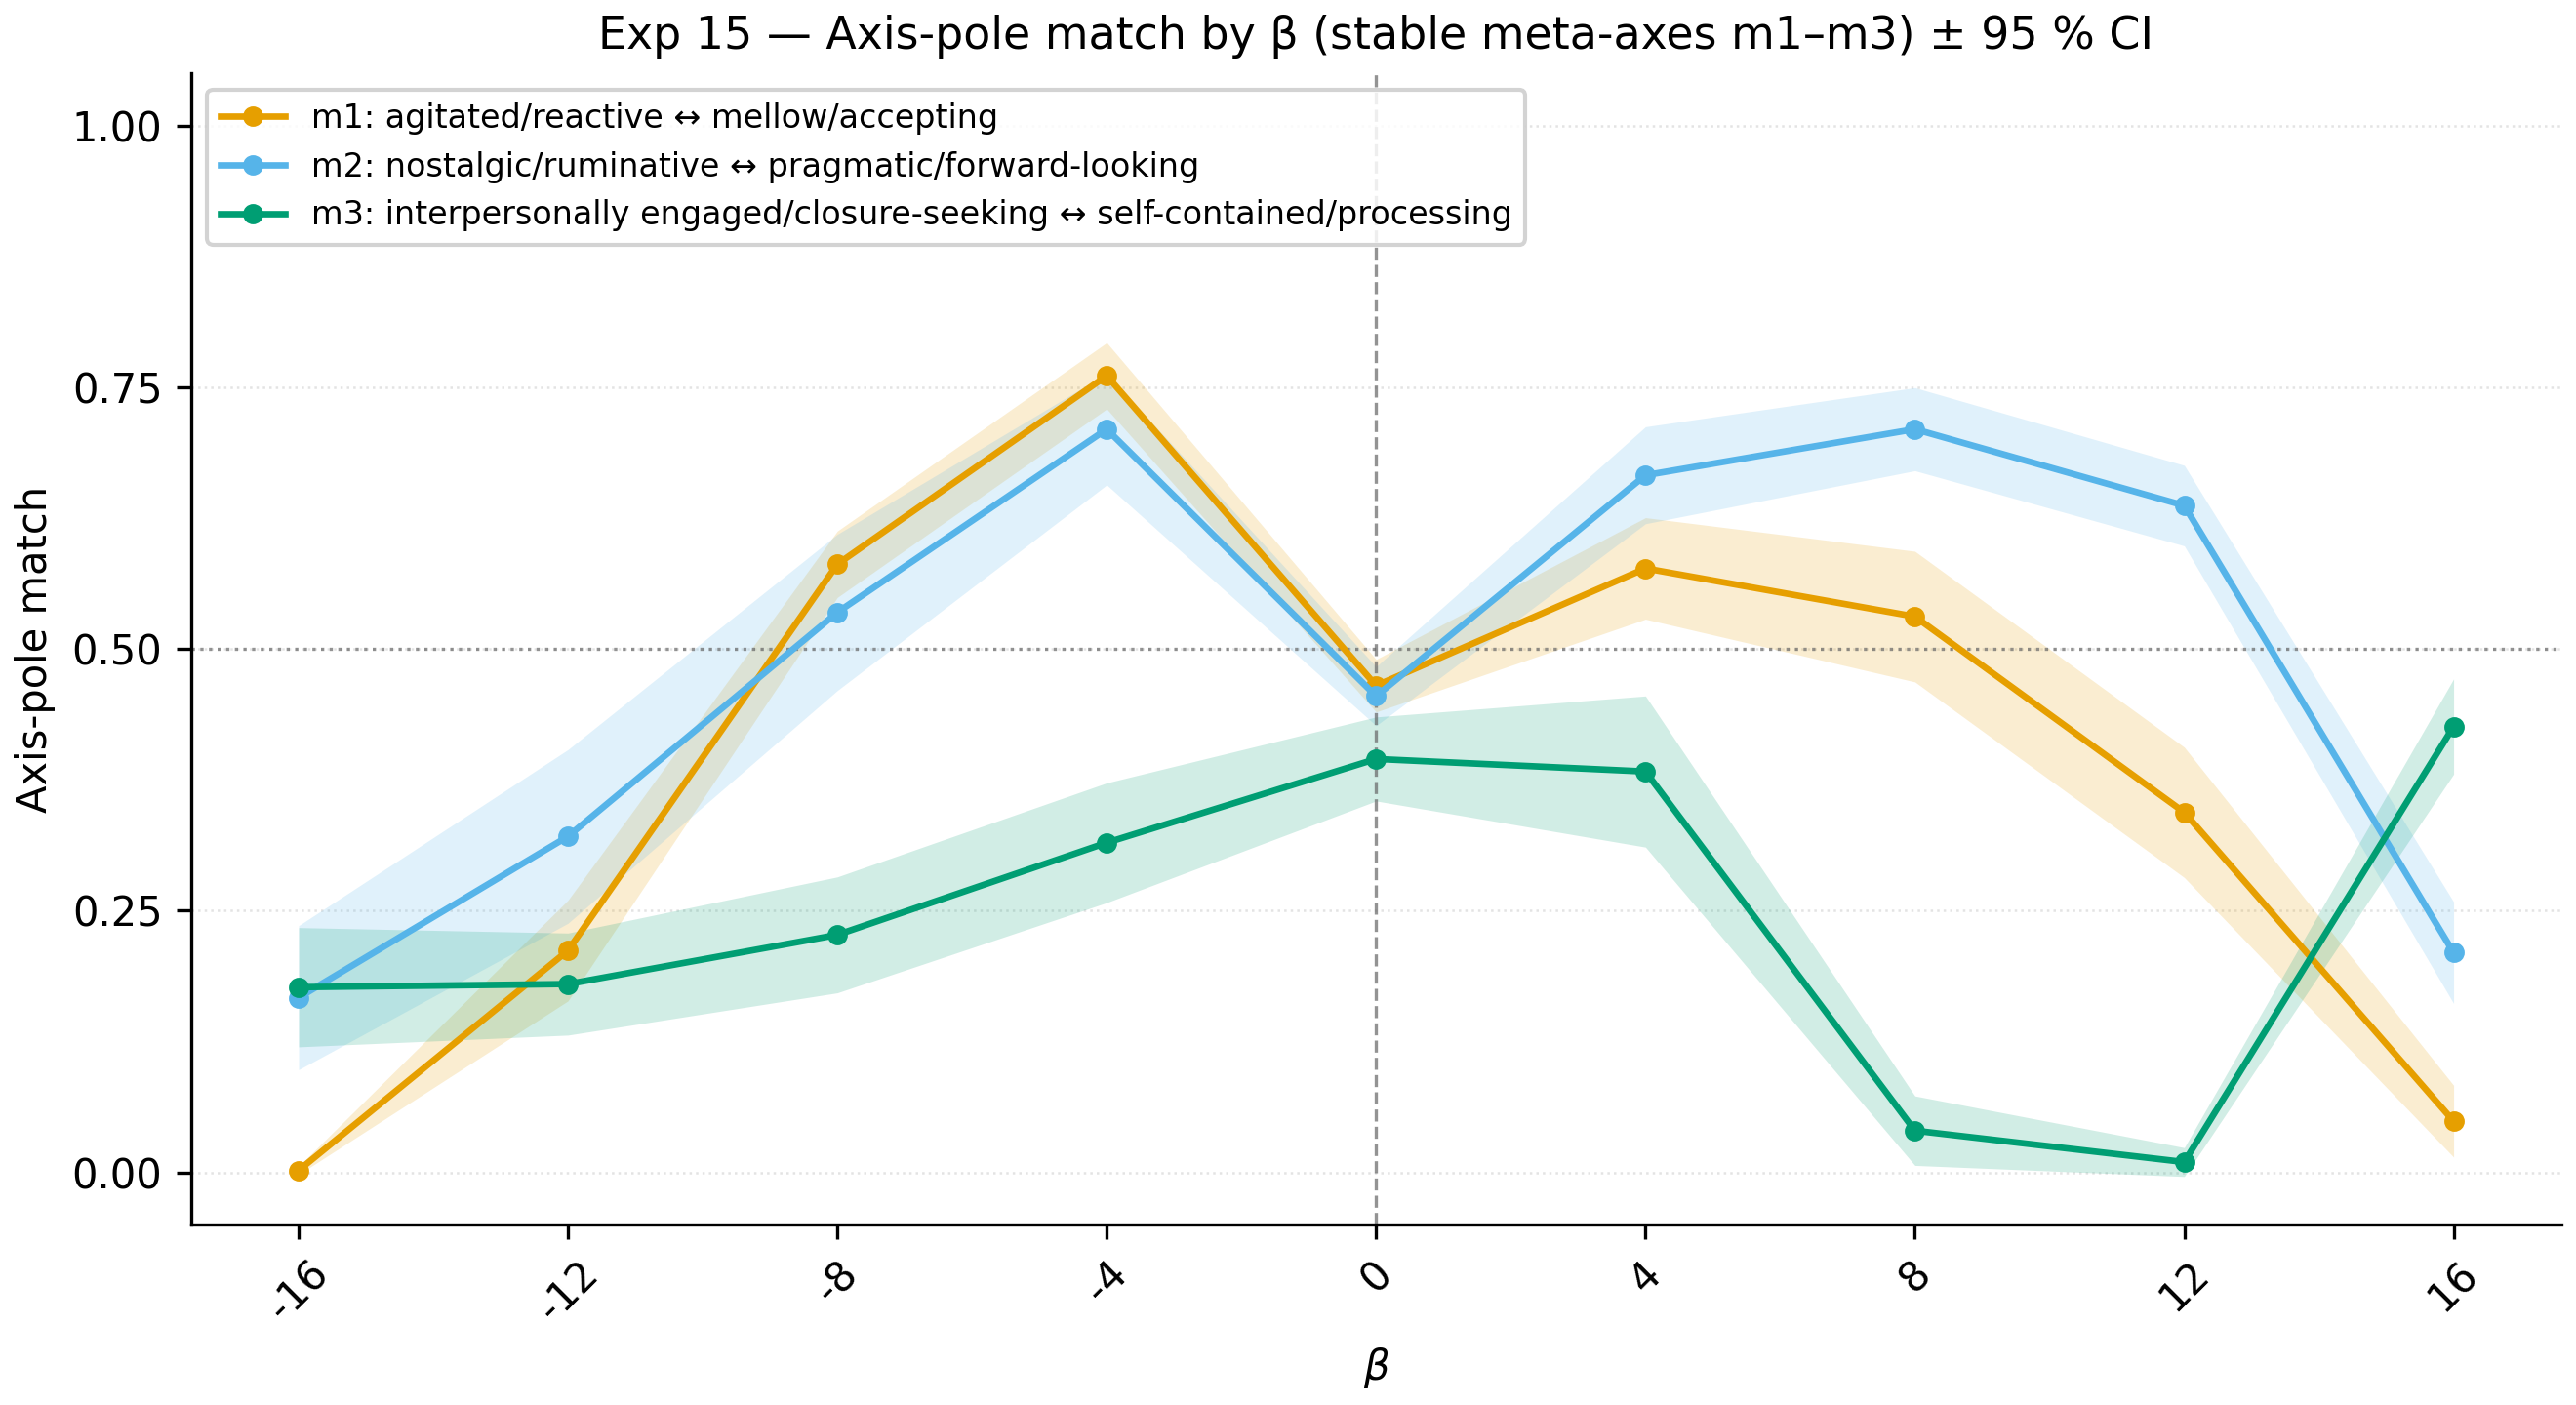
\includegraphics[width=0.7\linewidth]{figures/exp15_fig2_pole_match_stable_axes.png}
  \caption{3つの安定したメタ軸 $\mathbf{m}_1$--$\mathbf{m}_3$ のステアリング係数 $\beta$ の関数としての極マッチ率（$N=100$、95\% CI）。垂直破線はステアリングなしのベースライン（$\beta=0$）を示す。$\mathbf{m}_1$ と $\mathbf{m}_2$ が $\beta=-4$ で急峻なピークを示す一方、$\mathbf{m}_3$ はコヒーレントステアリングウィンドウ全体にわたってステアリングなしのベースライン付近に留まる。}
  \label{fig:exp15_stable_axes}
\end{figure}

Figure~\ref{fig:exp15_stable_axes} は $\mathbf{m}_1$ と $\mathbf{m}_2$ の両方が堅固なステアリング応答を示すことを示す。ここで、$\mathbf{m}_1$ は agitated/reactive $\leftrightarrow$ mellow/accepting に対応する。$\mathbf{m}_2$ は nostalgic/ruminative $\leftrightarrow$ pragmatic/forward-looking に対応する。\par
両軸ともステアリングなしのベースラインではほぼ偶然の値に近い位置にある。ベースラインの極マッチスコアは pm@0 $= 0.46$--$0.47$ である。$\beta=-4$ でのステアリングにより、極マッチは $\mathbf{m}_1$ で $0.761$、$\mathbf{m}_2$ で $0.710$ に向上する。これらは $+0.26$--$+0.30$ の絶対的な向上に対応する。\par
効果はコヒーレントステアリングウィンドウ内で発生する。これらのウィンドウは $\mathbf{m}_1$ で $[-8,16]$、$\mathbf{m}_2$ で $[-16,12]$ である。両ウィンドウ全体にわたって、soundness は $\geq 0.94$ に留まる。意味保存も $\geq 0.97$ に留まる。これは情動シフトが流暢性や命題的内容を劣化させないことを示す。\par
\texttt{subtle\_affective\_shift} スコアはスイープ全体にわたって極マッチを密接に追跡する。これは観察された変化が前言語的な表現のシフトを反映していることを確認する。したがってこれは感情カテゴリの置換ではなく、情動テクスチャの変化として理解される。\par

$\mathbf{m}_3$（interpersonally engaged $\leftrightarrow$ self-contained/processing）については僅かな向上のみが見られる。\texttt{pm}$_\text{peak}$ $= 0.426$（$\beta=+16$）で、ステアリングなしのベースライン $0.395$ より $+0.031$ 上である（Figure~\ref{fig:exp15_stable_axes}）。対人的志向性は層~13での単一テキスト継続ステアリングで確実にアクセスできないと推測される。これはコヒーレントウィンドウ $\beta \in [-12, 16]$ 全体にわたってほぼ平坦な極マッチ曲線と整合している。\par

\begin{table}[H]
\centering
\small
\begin{tabular}{llrrrrrr}
\toprule
\textbf{軸} & \textbf{安定性} & $L_\beta$ & $R_\beta$ & $M_A$ & pm@0 & \texttt{pm}$_\text{peak}$ & $\beta_\mathrm{peak}$ \\
\midrule
$\mathbf{m}_1$ & stable & $-8$  & $16$ & $4.0$  & 0.465 & \textbf{0.761} & $-4$ \\
$\mathbf{m}_2$ & stable & $-16$ & $12$ & $-2.0$ & 0.455 & \textbf{0.710} & $-4$ \\
$\mathbf{m}_3$ & stable & $-12$ & $16$ & $2.0$  & 0.395 & 0.426          & $+16$ \\
$\mathbf{m}_4$ & low    & $-16$ & $8$  & $-4.0$ & 0.345 & 0.563          & $-4$ \\
$\mathbf{m}_5$ & low    & $-8$  & $12$ & $2.0$  & 0.420 & \textbf{0.812} & $+4$ \\
\bottomrule
\end{tabular}
\caption{各メタ軸のコヒーレントウィンドウ（$L_\beta$、$R_\beta$）、ウィンドウ中心 $M_A$、ベースライン極マッチ pm@0、ピーク極マッチ \texttt{pm}$_\text{peak}$、および最適 $\beta$（$N=100$）。太字エントリは \texttt{pm}$_\text{peak}$ $\geq 0.70$ の軸を示す。}\label{tab:exp15_n100_summary}
\end{table}

抽出時の低安定性フラグにもかかわらず、$\mathbf{m}_5$（relief/release $\leftrightarrow$ tension/constraint）は $0.812$（$\beta=+4$；Table~\ref{tab:exp15_n100_summary}）ですべての軸の中で最も高い \texttt{pm}$_\text{peak}$ を達成する。$N=100$ のテキストは状況的・身体的状態の自然な描写を含んでおり、この身体的次元と特によく整合し、異常にクリーンなステアリング信号を生じさせると推測される。コヒーレントウィンドウは $\beta \in [-8, 12]$ である。\par

$\mathbf{m}_4$（mundane/obligatory $\leftrightarrow$ meaningful/fulfilling）は $\beta=-4$（LOW極；Table~\ref{tab:exp15_n100_summary}）で \texttt{pm}$_\text{peak}$ $= 0.563$ に達するが、HIGH極（$\beta > 0$）はほぼゼロの極マッチを示し、極間に顕著な非対称性が明らかになる。これは $\mathbf{m}_4$ のラベル割り当てが因果的効果と符号が一致していない可能性を示唆しており、これはその低い手法間安定性を考えると驚くべきことではない。\par

すべての軸において、コヒーレントウィンドウは $|\beta| \lesssim 12$--$16$ に限定される（Table~\ref{tab:exp15_n100_summary}）。境界では soundness が急速に劣化する（$\beta=-16$ での $\mathbf{m}_1$ で soundness $= 0.046$；$\beta=16$ での $\mathbf{m}_4$ で soundness $= 0.041$）。この劣化は使用可能なステアリング大きさの経験的上限を提供し、保守的なデフォルトとして $|\beta| \leq 8$ の使用を促す。\par

% move to appendix?
% \begin{figure}[H]
%   \centering
%   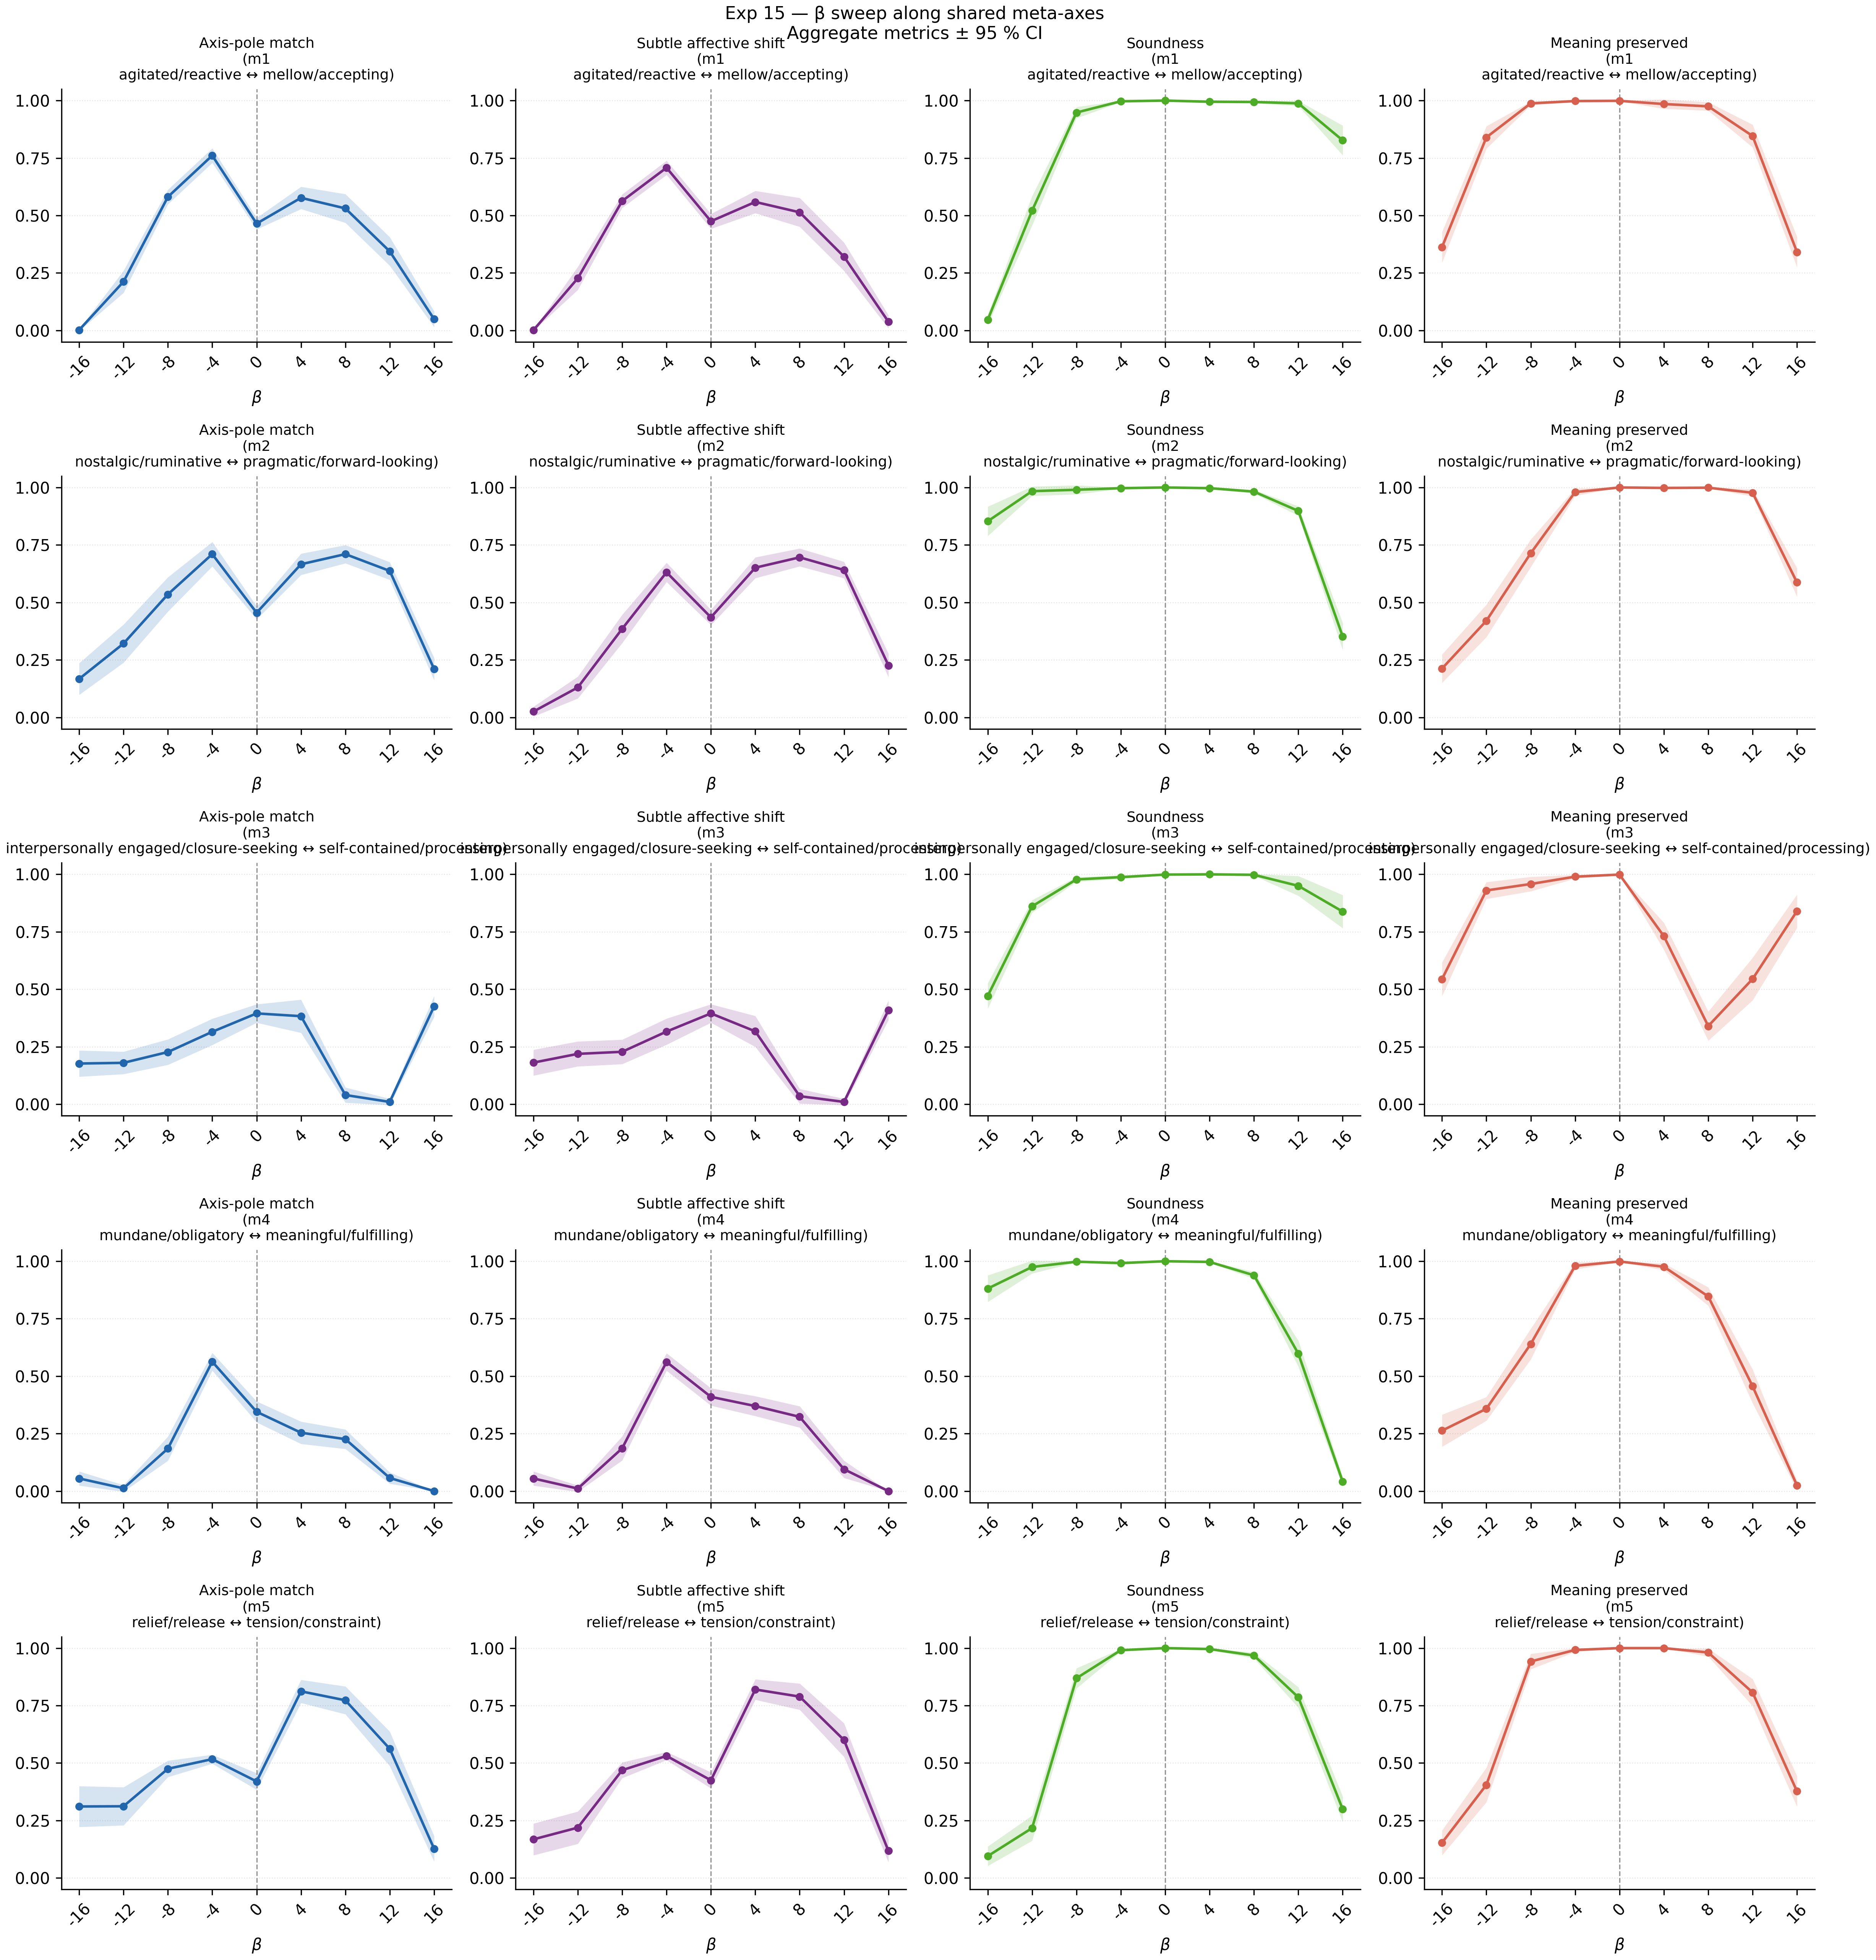
\includegraphics[width=\linewidth]{figures/exp15_fig1_aggregate_metrics_per_axis.png}
%   \caption{5つのメタ軸それぞれについての $\beta$ の関数としての4つすべての審判指標（$N=100$、95\% CI）。行は軸 $\mathbf{m}_1$--$\mathbf{m}_5$ に対応し、列は軸極マッチ、微細な情動シフト、soundness、および意味保存を示す。コヒーレントウィンドウ（soundness $\geq 0.70$）は各軸の有効な動作範囲を定義する。}
%   \label{fig:exp15_aggregate}
% \end{figure}

\subsection{定性的結果}
\label{sec:ch2-meta-axis-qualitative}

Table~\ref{tab:meta_axis_fear_m1} は\textit{fear}を表現するシード文が $\mathbf{m}_1$（\textit{agitated/reactive} $\leftrightarrow$ \textit{mellow/accepting} 軸）に沿ったステアリングによってどのように変調されるかの代表的な例を示す。3つのパターンが見られる。\par

正の $\beta$ は感情ラベルを変えることなく\textit{fear}の内臓的強度を高める。$\beta=4$ では、命題的内容はステアリングなしのベースライン（$\beta=0$）とほぼ同一である。同じ床のきしみが残る。同じ古い邸宅が残る。同じ不安を拭えないという感覚も残る。変わるのは情動的レジスターである。\textit{on edge}というフレーズと\textit{utterly unable to shake off}という構文は、ベースラインの\textit{breathless and unable to shake off the feeling}よりも反応をより即座で身体的なものにする。$\beta=8$ では感覚がさらにエスカレートする。床板が\textit{reverberate through every fiber of my being}する。\textit{Trepidation courses through my very soul}する。不安も\textit{refuses to subside}する。\textit{fear}はもはや単なる状況的な警告ではない。それは容赦のない身体的状態になる。このパターンは Section~\ref{sec:steering_causal_validation} で分析された $\hat{\mathbf{r}}_e$ ステアリングとは質的に異なる。$\alpha_R$ を増やすと感情カテゴリが変わる。例えば\textit{sadness}から\textit{anger}へ。対照的に、$\beta$ を増やすと固定された感情の中で情動テクスチャがシフトする。シフトは抑制された不安から内臓的な反応的恐怖へと向かう。\par

\begin{table}[H]
\centering
\small
\begin{tabular}{p{0.15\linewidth} p{0.78\linewidth}}
\toprule
\textbf{条件} & \textbf{ステアリング出力} \\
\midrule
\multicolumn{2}{l}{\textit{ベース：} Every creak of the floorboard made my heart race and I could not calm down.} \\
\midrule

$\beta = -4$
&
The eerie silence was shattered by every creak of the floorboard, making my heart skip a beat and my anxiety spike, but I couldn't shake the feeling that I was being watched. \\

\midrule

$\beta = 0$
&
As I stepped into the old mansion, every faint creak of the floorboard beneath my feet sent a jolt of anxiety coursing through my veins, leaving me breathless and unable to shake off the feeling of unease that had taken hold of me. \\

\midrule

$\beta = 4$
&
As I stepped into the old mansion, the faintest creak of the floorboards beneath my feet sent a jolt of anxiety coursing through my veins, leaving me on edge and utterly unable to shake off the sense of unease that had taken hold of me. \\

\midrule

$\beta = 8$
&
The mere sound of the floorboards beneath my feet seemed to reverberate through every fiber of my being, sending a jolting sense of trepidation coursing through my very soul, leaving me utterly consumed by an unrelenting sense of anxiety that refused to subside. \\

\midrule

$\beta = 16$
&
It seems that the statement is conveying that you are experiencing intense emotions, but it is clear that the statement is expressing your feelings in a concise and straightforward manner. \\

\bottomrule
\end{tabular}
\caption{ベース文「Every creak of the floorboard made my heart race and I could not calm down」を $\mathbf{m}_1$（\textit{agitated/reactive} $\leftrightarrow$ \textit{mellow/accepting}）でステアリングした例。正の $\beta$ は agitated/reactive の高極に向けてステアリングし、負の $\beta$ は mellow/accepting の低極に向けてステアリングする。}
\label{tab:meta_axis_fear_m1}
\end{table}

負の $\beta$ は感情ラベルを保持しながら出力を mellow/accepting 極に向けてステアリングする。$\beta=-4$ では同じ状況が続く。床板がきしみ、話者は見られているという感覚を払拭できない。しかし反応は質的に和らいでいる。元の文の\textit{``heart race''}は\textit{``heart skip a beat''}になる。不安はスパイクとして認識されるが、すぐに諦めのような譲歩的な\textit{``but I couldn't shake the feeling that I was being watched''}が続く。\textit{fear}は存在するが、抵抗されるのではなく受け入れられており、これは命名感情に変化がないことに対応しない区別である。これは $\mathbf{m}_1$ が前言語的テクスチャ軸として機能するという解釈を支持する。それはどの感情が存在するかではなく、感情がどのように保持され表現されるかを変調する。$\hat{\mathbf{r}}_e$ ステアリングとの対比は示唆的である。負の $\alpha_R$ は目標感情を抑制して対立するカテゴリに情動を向け直すが、負の $\beta$ はカテゴリ置換なしに同じ\textit{fear}をより諦めた、受容的な質に向けてシフトする。\par

過度な介入は $\hat{\mathbf{r}}_e$ で観察されたものとは異なる失敗モードを通じて生成品質を劣化させる。$\beta=16$ では、出力はステアリングされた文ではなくメタコメンタリーを生成する。\textit{``It seems that the statement is conveying that you are experiencing intense emotions''}。モデルは一人称の体験的モードを完全に終了し、表現的レジームの外側から語る。この視点の崩落は高い $\alpha_R$ で観察される語彙的反復ループとは質的に異なる。品質は $\beta=16$ で目に見えて劣化しており、これはコヒーレントウィンドウの端付近の極端な値が soundness と意味保存を低下させることを示すより広いスイープと整合している。\par

\subsection{解釈}

ステアリング実験から3つの結論が導かれる。第一に、メタ軸は因果的に活性である。$\beta\,\mathbf{m}_k$ を直接注入することで、中程度のステアリング大きさで一貫した、審判が検証した情動テクスチャのシフトが生成される。\par

第二に、効果はテクスチャ固有である。\texttt{pm} スコアは \texttt{subtle\_affective\_shift} を密接に追跡する。同時に、意味保存はコヒーレントウィンドウ内で高く保たれる。これはシフトが表現の「何」ではなく「どのように」にあることを示す。\par

第三に、因果的効果は軸依存である。$\mathbf{m}_3$ は幾何学的に安定しているが、コヒーレントウィンドウ全体にわたってステアリングに抵抗する。これは幾何学的回復可能性が単層での因果的制御可能性を保証しないことを示唆する。対人的志向性は覚醒度や時間的志向性よりも単一の残差ストリーム層に局所化されていないと推測される。これを確認するには現在の実験の範囲を超えた多層アブレーションが必要である。Appendix~\ref{app:ablation}（A2）は $\beta=0$ ベースラインが部分的偽証制御として機能する程度を論じ、ランダム方向注入実験を残された検証ステップとして特定する。\par

これらの結果はこの章の議論を完成させる。少なくとも $\mathbf{m}_1$ と $\mathbf{m}_2$ は前言語的情動次元と相関した単なる幾何学的構造ではない。現在のデータセットでは、低安定性軸 $\mathbf{m}_5$ も因果的に振る舞う。これらの軸は感情ラベルを変えることなく感情表現のテクスチャをシフトするように独立して操作できる。\par
したがってステアリング式は次のようになる。
\[
\Delta_e \;=\; \alpha_R\,\hat{\mathbf{r}}_e \;+\; \sum_{k}\gamma_k\,\mathbf{m}_k,
\]
ここで2つの項は機能的に分離可能である。係数 $\alpha_R$ は感情アイデンティティを制御する。係数 $\gamma_k$ は前言語的情動テクスチャを変調する。\par
